\section{Evaluation}
\subsection{Signal Strength Threshold}
Once we build a basic service flow, we needed to set up the threshold of Bluetooth signal strength to determine when the system will open up the gate depending on how far the user is. Since we presumed that the distance to user from the parking lot gate attached to Bluetooth module is correspond the signal strength, we needed empirical data of signal strength to evaluate the system efficiency and stability.

Thus, we performed experiments to collect signal stre-ngth of Bluetooth with the android device after setting up a practical environment outside. We put the two cars in a row and collected signal strength inside of each car, first car in front and second car behind.

Figure~\ref{fig:comparison} shows the comparison between the collected data for 60 seconds in the first car and the second car. As a result of plentiful of experiment, 10 minutes * 3 times in a day * 3 days, we observed that the range of signal strength in the first car was -67 to -80 and -88 to -96 (or less) and the median was -72 and -90 (Bold lines).

Based on the analysis, we set the threshold at -85 and it returned desirable result to an extend that it prevents perfectly for even a corner case problem that unregistered user in front gets in to the gate piggybacking the grant of user behind. What it means is the system only opens the gate for the user who is within a range of about a car length.
\subsection{Discovery Latency}
In addition, to evaluate the performance of our system regarding latency, we also measured waiting time to open the gate, while the vehicle is in motion and in stillness. Through this experiment, we observed that the waiting time is truly random whether the vehicle is moving or not. This is because the Bluetooth discovery process in Android usually takes 12 seconds of inquiry scan cycle \cite {btcycle}. In order words, at any moment during 12 seconds, the Bluetooth module can be found and the user might have no waiting time to 12 seconds of waiting time, at most.

\begin{figure}
	\centering
	\begin{subfigure}[b]{.5\linewidth}
		\centering
		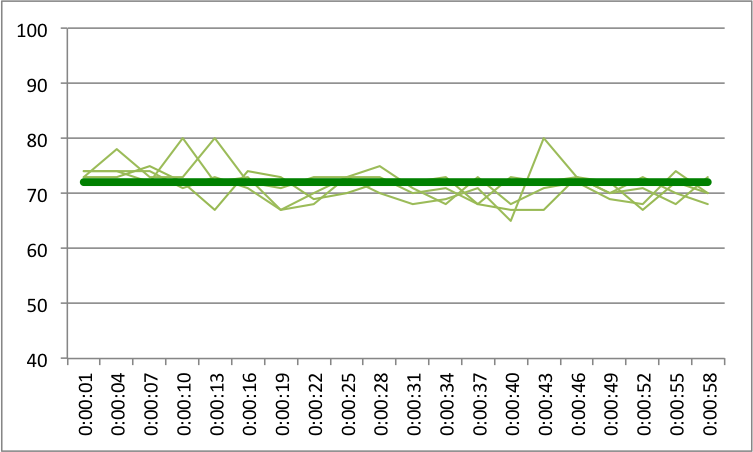
\includegraphics[width=1.5in]{figure/bt_first_car}
		\caption{The first car in front}
		\label{fig:first car}
	\end{subfigure}%
	\begin{subfigure}[b]{.5\linewidth}
		\centering
		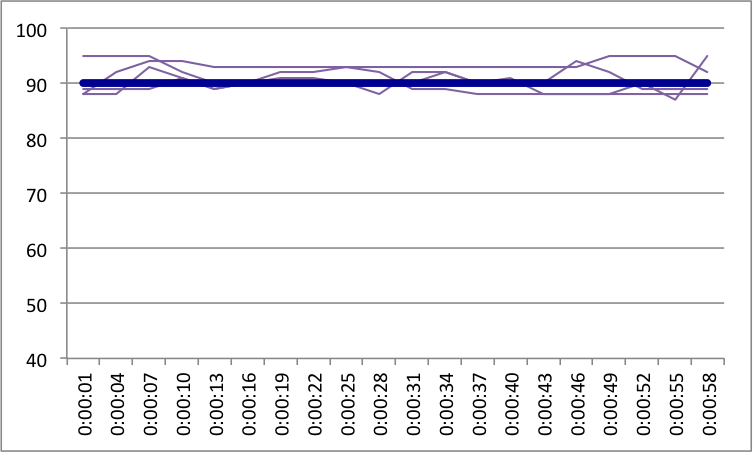
\includegraphics[width=1.5in]{figure/bt_second_car}
		\caption{The second car behind}
		\label{fig:second car}
	\end{subfigure}
	\caption{RSSI Comparison between two cars}
	\label{fig:comparison}
\end{figure}

This limitation made us cannot use average value of multiple samples to set up the threshold. Since, suppose, we want to collect 5 samples for averaging out, then the user has to wait 60 seconds in worst-case scenario.
